% https://www.mathcha.io/editor# использован для построения картинок

\tikzset{every picture/.style={line width=0.75pt}} %set default line width to 0.75pt        

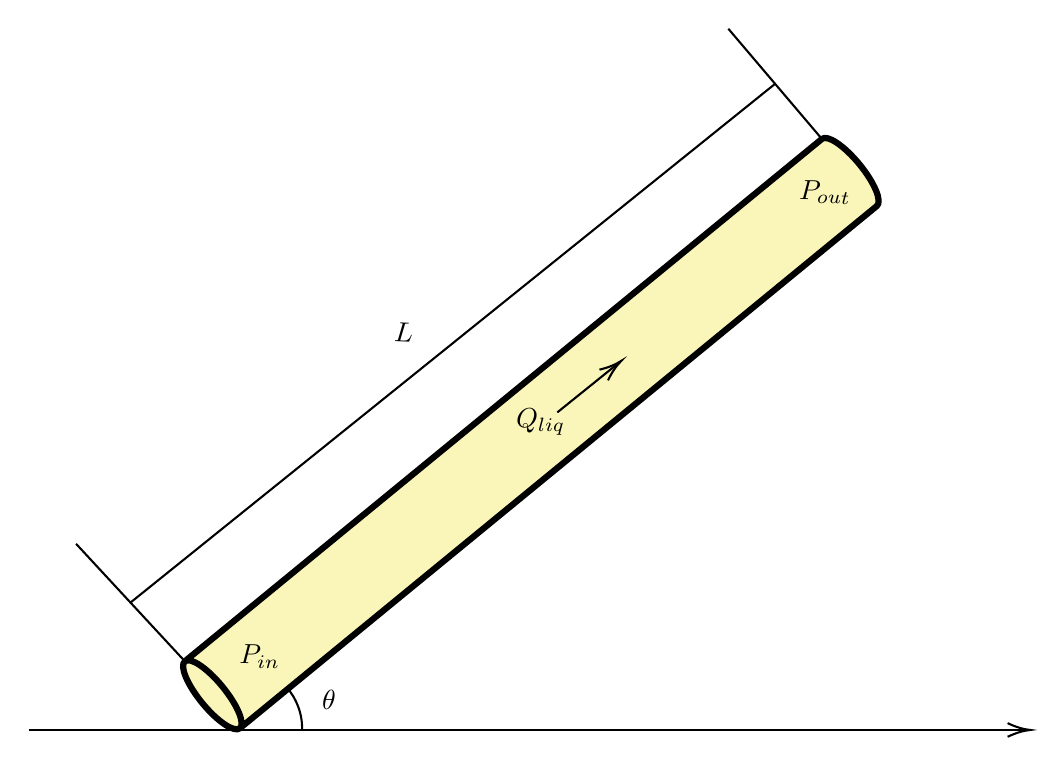
\begin{tikzpicture}[x=0.75pt,y=0.75pt,yscale=-1,xscale=1]
%uncomment if require: \path (0,395.3333282470703); %set diagram left start at 0, and has height of 395.3333282470703

%Shape: Can [id:dp2899696286091056] 
\draw  [fill={rgb, 255:red, 250; green, 245; blue, 184 }  ,fill opacity=1 ][line width=2.25]  (164.23,345.91) -- (471.15,94.25) .. controls (473.82,92.06) and (481.92,97.51) .. (489.23,106.43) .. controls (496.54,115.34) and (500.3,124.35) .. (497.63,126.55) -- (190.71,378.2)(164.23,345.91) .. controls (166.9,343.71) and (175,349.16) .. (182.31,358.08) .. controls (189.63,367) and (193.39,376.01) .. (190.71,378.2) .. controls (188.03,380.4) and (179.94,374.95) .. (172.62,366.03) .. controls (165.31,357.11) and (161.55,348.1) .. (164.23,345.91) -- cycle ;
%Shape: Arc [id:dp7673222576415257] 
\draw  [draw opacity=0] (213.54,358.73) .. controls (215.72,361.29) and (217.51,364.25) .. (218.76,367.57) .. controls (220.22,371.43) and (220.84,375.4) .. (220.7,379.27) -- (190.71,378.2) -- cycle ; \draw   (213.54,358.73) .. controls (215.72,361.29) and (217.51,364.25) .. (218.76,367.57) .. controls (220.22,371.43) and (220.84,375.4) .. (220.7,379.27) ;
%Straight Lines [id:da2539925089352497] 
\draw    (111.83,289.33) -- (164.23,345.91) ;


%Straight Lines [id:da27080386920459176] 
\draw    (426.06,41.14) -- (471.15,94.25) ;


%Straight Lines [id:da6784647335940455] 
\draw    (138.03,317.62) -- (448.6,67.7) ;


%Straight Lines [id:da42906958912244875] 
\draw    (343.67,226) -- (373,202.37) ;
\draw [shift={(374.56,201.11)}, rotate = 501.14] [color={rgb, 255:red, 0; green, 0; blue, 0 }  ][line width=0.75]    (10.93,-3.29) .. controls (6.95,-1.4) and (3.31,-0.3) .. (0,0) .. controls (3.31,0.3) and (6.95,1.4) .. (10.93,3.29)   ;

%Straight Lines [id:da31602361859897776] 
\draw    (89,379) -- (569.56,379) ;
\draw [shift={(571.56,379)}, rotate = 180] [color={rgb, 255:red, 0; green, 0; blue, 0 }  ][line width=0.75]    (10.93,-3.29) .. controls (6.95,-1.4) and (3.31,-0.3) .. (0,0) .. controls (3.31,0.3) and (6.95,1.4) .. (10.93,3.29)   ;


% Text Node
\draw (233.67,364.33) node   {$\theta $};
% Text Node
\draw (269.67,187.67) node [rotate=-2.44]  {$L$};
% Text Node
\draw (200.33,343.67) node [rotate=-0.74]  {$P_{in}$};
% Text Node
\draw (472.67,120) node [rotate=-0.74]  {$P_{out}$};
% Text Node
\draw (335.67,230.67) node [rotate=-0.61]  {$Q_{liq}$};


\end{tikzpicture}